\chapter{Introduction}

Cada dia el nombre de transaccions amb efectiu es van reduïnt. Els diners en efectiu ocupen espai i, sobretot les monedes, pesen molt. És per això que les transaccions s'encaminen cap al \textit{cashless} (en anglès, sense efectiu).



Technological developments in Electronics and Signal Processing fields are also being implemented in the nowadays manufactured vehicles. A considerable number of the vehicle functions have moved to be controlled by electronic actuators. This is the case of, for example, fuel valves, brakes, door and windows opening/closing, etc. In addition, most vehicles are including an on-board computer that monitors all the vehicle parameters --speed, remaining fuel, range, etc.--, and inform the driver about any detected potential danger. All those systems that help the driver and made a safer driving are known as DAS, Driving Assistant Systems.

Recently, a new group of technological   developments for the automotive industry has sprung: the Advanced Driving Assistance Systems (ADAS). This category embraces those advanced systems that offer the driver a guidance about the environment of the vehicle. Some known examples are parking assistant --ultrasound system that alerts the driver when the rear distance to an object is below a certain limit--, lane departure warning -alerts the driver when any wheel crosses a lane delimiter line-, traffic assistance --the vehicle detects and interprets the traffic signals--, among others.

This project will focus on a specific ADAS: 360\degree~vision system. These device range offer the driver a complete top view --or bird's eye view-- of the vehicle surroundings, allowing the driver to see through blind spots around the vehicle. The most common set-up  includes several cameras located around the vehicle, and a display where the driver can view a composite image made from the camera data.  

360\degree~vision systems, also called bird's eye systems, are currently offered in high-end passenger cars. This systems can be combined with other features such as lane departure warning or pedestrian detection. Figure~\ref{fig:intro-example} shows two screenshots from different commercial 360\degree~vision systems. 

\begin{figure}
	\centering
	\begin{subfigure}[b]{0.45\textwidth}
		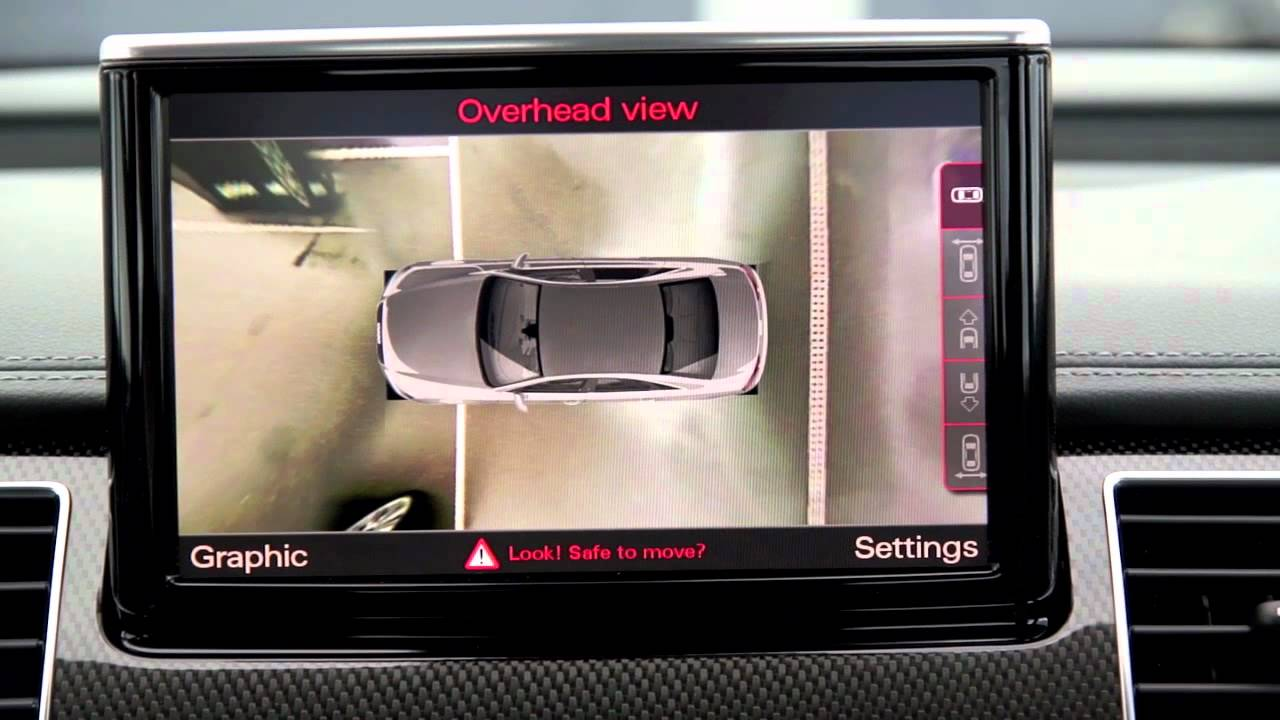
\includegraphics[width=\textwidth]{images/audi-intro}
		\caption{Audi S8 -- 360 View Camera}
		\label{fig:audi-intro-example}
	\end{subfigure}
	\hspace{0.5cm}
	\begin{subfigure}[b]{0.45\textwidth}
		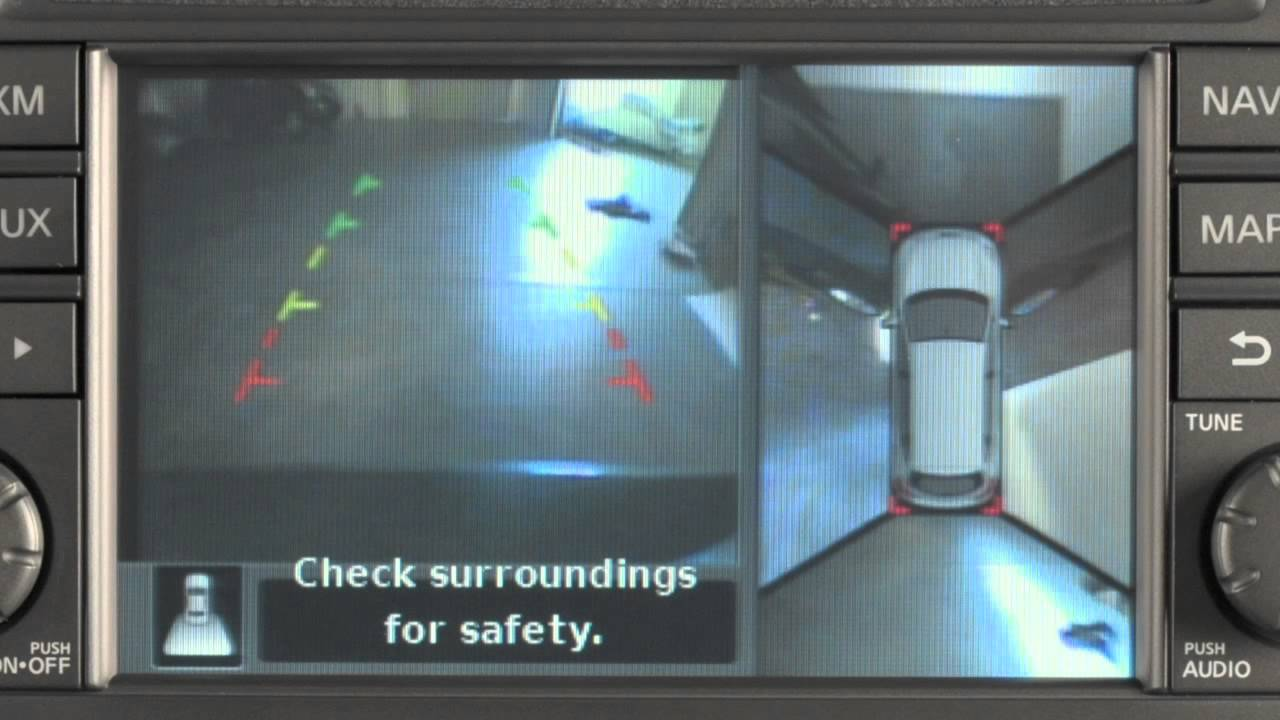
\includegraphics[width=\textwidth]{images/nissan-intro}
		\caption{Nissan Rogue -- Around View Monitor}
		\label{fig:nissan-intro-example}
	\end{subfigure}
	\caption{Two commercial 360\degree~vision systems display view}
	\label{fig:intro-example}
\end{figure}

However, 360\degree~vision system for passenger cars can not be straightforwardly applied to all vehicle types. The camera amount, its position, the vehicle length and height and the ROI (Region of Interest) make this algorithms specifically adapted to a vehicle type. Thus, the aim of this project will be to develop an 360\degree~vision systems for long vehicles, specifically buses. 

This vision system is an specific part of the work commissioned by the company Arcol to a multidisciplinary UPC team. Arcol is a mirrors and accessories manufacturer for motorhomes, buses and coaches. Currently, this company is working jointly with the UPC in a 3-year project. This project main goal is to develop a camera-and-display based guidance system for the driver.

This project is carried out jointly in two UPC research groups: The Image Processing Group (GPI) and the Advanced Hardware Architecture (AHA) group. The AHA group main tasks are, on a high profile, to develop all the hardware to obtain and process the signals. The Image Processing Group is responsible of the computer vision algorithms development. During this project first year, the AHA group is developing the recording/display drivers and programming the hardware accelerators needed. Meanwhile, the GPI group is developing the 360\degree~vision system and a pedestrian detection system.

This TFG project contains the part of the work developed in the Image Processing Group developing the  360\degree~vision system, focusing on the image warping algorithms. Thus, this project also develops several parts corresponding to other stitching stages. Stitching algorithm parts developed by other GPI team members, and therefore outside the scope of this project, are only briefly stated for a whole stitching algorithm understanding.

\section{Project goals}
The work done in the Image Processing Group started on February 2014. As stated on the Project Proposal and Workplan delivered on February 14th, this TFG work will end at June 30th, although the work in the ARCOL project will be still in development until December 2014.

This project goals had been defined before the development began, and are stated in the Project Proposal and Workplan mentioned above. The goals of this project can be summed up in the following points:
\vspace{-0.5em}
\begin{description}[font=\normalfont\textsl]
\item [Representative points automatic detection.] To perform the stitching a reference points set had to be highlighted on the image. One of this project goals is to define this points and the model shown to each camera on the calibration step.
\item [Estimate the warping parameters. ] Study the most suitable transformation and the parameters needed to deform the input images to obtain the output stitched image.
\item [Blending the results on the final stitching. ] Define an algorithm to merge the warped images on the final composition.
\item [Follow the requirements stated by the Arcol project. ]All the procedures stated before have to be done according with the Arcol UPC project requirements. This requirements and specifications can be found in Chapter~\ref{chapter:requirements}. 
\end{description}

The work done in this five months has been focused on developing a proper warping algorithm for this specific environment, taking into account all the technical an logistic issues. The specific tasks that had been included in  this project scope are explained in Chapter~\ref{chapter:methodology}.

\section{Time Plan}
The time plan followed during this project development is shown in Figure~\ref{fig:gantt} Gantt Diagram. The developed work has been split in 8 work packages. A detailed description of each work package and the internal tasks developed can be found on Appendix~\ref{app:gantt}. 

\begin{figure}[ht]
\center
\begin{ganttchart}[
hgrid,
bar/.append style={fill=blue!50},
vgrid={*4{dotted},*1{dashed},*3{dotted},*1{dashed},*3{dotted},*1{dashed},*3{dotted},*1{dashed},*4{dotted},*1{dashed}},
x unit=0.47cm,
title height=1, 
y unit title=0.6cm,
y unit chart=0.8cm]{1}{27}
\gantttitle{Project timeline in months/weeks}{27} \\
\gantttitle[title label node/.append style={below left=-8pt and -30pt}]{{\footnotesize\textit{Month}}\quad JANUARY}{5}\gantttitle{FEBR.}{4}\gantttitle{MARCH}{4}\gantttitle{APRIL}{4}\gantttitle{MAY}{5}\gantttitle{JUNE}{5} \\
\gantttitle[title label node/.append style={below left=-8pt and -7pt}]{\footnotesize\textit{Week}\quad1}{1}
\gantttitlelist
{2,...,27}{1} \\ 
\ganttbar{Documentation}{1}{5} \\
\ganttmilestone
{\emph{Captures}}{6}\ganttmilestone
{}{11}\ganttmilestone
{}{18}\\
%\ganttbar{Captures}{6}{6}\ganttbar{}{11}{11}\ganttbar{}{18}{18} \\
\ganttbar{Undistortion}{6}{7}\ganttbar{}{11}{17} \\
\ganttbar{Registering}{18}{20} \\ 
\ganttbar{Warping}{8}{10}\ganttbar{}{15}{23} \\
\ganttbar{Blending}{10}{10}\ganttbar{}{22}{23} \\
\ganttbar{Optimization}{23}{24} \\
\ganttbar{Writing}{22}{27}
\end{ganttchart}
\caption{Project Gantt Chart}
\label{fig:gantt}
\end{figure}








